\chapter{Monte Carlo Synthetic Acceleration Methods for the
  Navier-Stokes \\Equations\ }
\label{ch:nonlinear_problem}
Nonlinear transport problems are a common occurrence in single and
multiple physics problems in nuclear engineering. Systems of partial
differential equations, such as the Navier-Stokes equations that
describe fluid flow, yield discrete sets of stiff equations with
nonlinearities present in the variables when discretized by
conventional methods. These sets of equations characterize momentum
and energy transport through diffusion, viscous forces, and inertial
forces. Traditionally, such systems have been solved by linearizing
them in a form where the nonlinearities in the variables are
eliminated and more traditional linear methods can be used for
solutions. Often characterized as segregated methods where physics
operators are split and their action on the system approximated in
steps, such methods lack consistency and accuracy in resolving the
nonlinear component of the solution. In the last 30 years, fully
consistent nonlinear methods based on Newton's method have become more
popular and many advances have been made in the nuclear engineering
field to employ these methods.

In the context of solving standalone linear systems, Monte Carlo
methods do not provide significant merit over subspace methods due to
the fact that the linear operator must be explicitly formed. For many
applications including higher fidelity neutron transport
discretizations beyond the $SP_N$ equations solved in the previous
chapter, such a requirement is prohibitive and perhaps not even
feasible to implement. Therefore, a discrete Monte Carlo solution
method is best suited for situations in which the operator is readily,
if not naturally, formed. Modern nonlinear methods meet this
requirement with Newton methods used in conjunction with Krylov
methods operating on a fully formed matrix for a robust solution
strategy. Furthermore, modern techniques exist that permit the
automatic construction of the Jacobian operator generated within a
Newton method based on the nonlinear residual evaluations, providing
all of the components necessary for a Monte Carlo solver to provide
value.

We therefore devise a new nonlinear method based on the MCSA algorithm
and Newton's method. In this chapter the fundamentals of Newton's
method will be presented along with a brief discussion of inexact
Newton methods. Newton-Krylov methods, a variant of inexact Newton
methods, will be outlined along with two common techniques for
Jacobian generation as a means of defining current
practices. Following this, the new algorithm will be presented and
implementation details will be discussed. Using the new algorithm and
a production fluid physics code, a group of challenging nonlinear
benchmark problems for the Navier-Stokes equations will be used to
verify the correctness of the method relative to solutions obtained
using conventional methods in various flow regimes. Finally, we will
compare the performance of the new method against contemporary
Newton-Krylov methods for the same benchmark problems.

%%---------------------------------------------------------------------------%%
\section{Preliminaries\ }
\label{sec:nonlinear_preliminaries}
We formulate the \textit{nonlinear problem} as follows
\citep{knoll_jacobian-free_2004}:
\begin{equation}
  \ve{F}(\ve{u}) = \ve{0}\:,
  \label{eq:nonlinear_problem}
\end{equation}
where $\ve{u} \in \mathbb{R}^n$ is the solution vector and
$\ve{F}:\mathbb{R}^N \rightarrow \mathbb{R}^N$ is the function of
nonlinear residuals. We write the nonlinear system in this form so
that when an exact solution for $\ve{u}$ is achieved, all residuals
evaluate to zero. \textit{Newton's method} is a root finding algorithm
and therefore we can use it to solve Eq~(\ref{eq:nonlinear_problem})
if we interpret the exact solution $\ve{u}$ to be the roots of
$\ve{F}(\ve{u})$. Newton's method is also an iterative scheme, and we
can generate this procedure by building the Taylor expansion of the
$k+1$ iterate of the nonlinear residuals about the previous $k$
iterate:
\begin{equation}
  \ve{F}(\ve{u}^{k+1}) = \ve{F}(\ve{u}^{k}) +
  \ve{F}'(\ve{u}^{k})(\ve{u}^{k+1}-\ve{u}^{k}) +
  \frac{\ve{F}''(\ve{u}^{k})}{2}(\ve{u}^{k+1}-\ve{u}^{k})^2 + \cdots
  \:.
  \label{eq:newton_derivation_1}
\end{equation}
If we ignore the nonlinear terms in the expansion and assert that at
the $k+1$ iterate $\ve{u}^{k+1}$ is the exact solution such that
$\ve{F}(\ve{u}^{k+1}) = \ve{0}$, then we are left with the following
equality:
\begin{equation}
  -\ve{F}(\ve{u}^{k}) =
  \ve{F}'(\ve{u}^{k})(\ve{u}^{k+1}-\ve{u}^{k})\:.
  \label{eq:newton_derivation_2}
\end{equation}
We note two things of importance in
Eq~(\ref{eq:newton_derivation_2}). The first is that
$\ve{F}'(\ve{u}^{k})$ is in fact the \textit{Jacobian},
$\ve{J}(\ve{u})$, of the set of nonlinear residuals and is defined
element-wise as:
\begin{equation}
  J_{ij} = \frac{\partial F_i(\ve{u})}{\partial u_j}\:.
  \label{eq:jacobian_def}
\end{equation}
Second, we note that $(\ve{u}^{k+1}-\ve{u}^{k})$ is simply the
solution update from the $k$ iterate to the $k+1$ iterate. We will
define this update as the \textit{Newton correction} at the $k$
iterate, $\delta \ve{u}^k$. To finish, we can then rearrange
Eq~(\ref{eq:newton_derivation_2}) to define the Newton iteration
scheme for nonlinear problems:
\begin{subequations}
  \begin{gather}
    \ve{J}(\ve{u}) \delta \ve{u}^k = -\ve{F}(\ve{u}^{k})\\
    \ve{u}^{k+1} = \ve{u}^k + \delta \ve{u}^k\:.
  \end{gather}
  \label{eq:newton_iteration}
\end{subequations}
There are then three distinct steps to perform: evaluation of the
nonlinear residuals using the solution at the $k$ iterate, the
solution of a linear system to compute the Newton correction where the
Jacobian matrix of the nonlinear equation set is the linear operator,
and the application of the correction to the previous iterate's
solution to arrive at the next iterate's solution. In the asymptotic
limit, the iterations of Newton's method will converge the nonlinear
residual quadratically \citep{kelley_iterative_1995}. Convergence
criteria is set for stopping the iteration sequence based on the
nonlinear residual. Commonly, the following criteria is used:
\begin{equation}
  ||\ve{F}(\ve{u}^{k})|| < \epsilon ||\ve{F}(\ve{u}^{0})||\:,
  \label{eq:newton_stopping_criteria}
\end{equation}
where $\epsilon$ is a user defined tolerance parameter. 

Newton's method is \textit{consistent} in that all components of the
nonlinear functions that describe the physics we are modeling are
updated simultaneously in the iteration sequence with respect to one
another. This is in comparison to \textit{inconsistent} strategies,
such as a pressure correction strategy for solving the Navier-Stokes
equations \citep{pletcher_computational_1997}, where the components of
$\ve{u}$ are updated in a staggered fashion depending on the
particular equations that they are associated with.

\subsection{Inexact Newton Methods}
\label{subsec:inexact_newton_methods}
Inexact Newton methods arise when the Jacobian operator is not exactly
inverted, resulting in an inexact Newton correction as initially
described by Dembo and others \citep{dembo_inexact_1982}. For common
sparse nonlinear systems, which in turn yield a sparse Jacobian
matrix, this situation occurs when conventional iterative methods are
applied. In their definition, Dembo formulated inexact methods such
that they are independent of the linear method used to solve for the
Newton correction and therefore are amenable to use with any linear
solver. Furthermore, they bind the convergence of the outer nonlinear
iteration to the inner linear iteration such that:
\begin{equation}
  ||\ve{J}(\ve{u}^k)\delta \ve{u}^k + \ve{F}(\ve{u}^k)|| \leq \eta^k
  ||\ve{F}(\ve{u}^k)||\:,
  \label{eq:inexact_newton_forcing}
\end{equation}
where $\eta^k \in [0,1)$ is defined as the \textit{forcing term} at
  the $k$ iterate. Eq~(\ref{eq:inexact_newton_forcing}) then states
  that the residual generated by the linear solver is bound by the
  nonlinear residual and how tightly it is bound is defined by the
  forcing term. This is useful in that we can vary how tightly coupled
  the convergence of the linear iterations used to generate the Newton
  correction is to the nonlinear iteration by relaxing or tightening
  the convergence properties on the linear iterative method. As a
  result, strategies for determining the forcing term can vary
  depending on the problem type and can greatly affect the convergence
  of the method or even prohibit convergence
  \citep{eisenstat_choosing_1996}. In addition, \textit{globalization
    methods} may be used to modify the Newton correction in a more
  desirable direction such that convergence properties can be
  improved when the initial guess for $\ve{u}$ is poor
  \citep{pawlowski_globalization_2006}.

\subsection{Newton-Krylov Methods\ }
\label{subsec:newton_krylov_methods}
A form of inexact Newton methods, \textit{Newton-Krylov methods} are
nonlinear iterative methods that leverage a Krylov subspace method as
the linear solver for generating the Newton correction
\citep{kelley_iterative_1995}. As outlined in
Appendix~\ref{ch:linear_problem}, Krylov methods are robust and enjoy
efficient parallel implementations on modern
architectures. Furthermore, their lack of explicit dependence on the
operator make them easier to implement than other
methods. Additionally, although many iterations can become memory
intensive due to the need to store the Krylov subspace for the
orthogonalization procedure, at each nonlinear iteration this cost is
reset as the Jacobian matrix will change due to its dependence on the
solution vector. This means that for every nonlinear iteration, a
completely new linear system is formed for generating the Newton
correction and we can modify the Krylov solver parameters accordingly
to accommodate this. In most nonlinear problems, the Jacobian operator
is generally non-symmetric and therefore either Krylov methods with
long recurrence relations that can handle non-symmetric systems must
be considered or the Newton correction system must be preconditioned
such that the operator is symmetric and short recurrence relation
methods can be potentially be used.

With many Krylov methods available, which to use with the Newton
method is dependent on many factors including convergence rates and
memory usage. Several studies have been performed to investigate this
\citep{mchugh_inexact_1993,knoll_newton-krylov_1995}. In their
numerical studies in 1995, Knoll and McHugh used the set of highly
nonlinear and stiff convection-diffusion-reaction equations to solve a
set of tokamak plasma problems with the goal of measuring solver
performance with Newton's method. They note several trade-offs in
using Krylov methods with the Newton solver. The first is that the
optimization condition that results from the constraints (e.g. the
minimization of the GMRES residual over the Krylov space) can be
relaxed by restricting the size of the subspace such that only a fixed
number of subspace vectors may be maintained, thus reducing memory
requirements. 

We can also relax the optimization condition by instead restarting the
recurrence relation with a new set of vectors once a certain number of
vectors have been generated. The optimization condition is maintained
over that particular set of vectors, however, Knoll and McHugh note
that this ultimately slows the convergence rate as compared to keeping
all vectors as the new set of vectors is not necessarily orthogonal to
the previous set, and therefore not optimal over the entire iteration
procedure. The orthogonality condition can be relaxed by using a
recurrence relation that does not generate a strictly orthonormal
basis for the Krylov subspace such as the Lanzcos biorthogonalization
procedure, resulting in memory savings due to the shorter Lanzcos
recurrence relation. Based on their numerical analysis, they observed
GMRES to be the most robust for any given nonlinear problem and
therefore used it for subsequent work in this area.

\subsection{Jacobian-Free Approximation}
\label{subsec:jacobian_free_approximation}
In many cases, the Jacobian is difficult to form from the difference
equations and costly to evaluate for large equation sets. For simple
nonlinear cases such as the Navier-Stokes equations, the derivatives
can be computed and coded, but due to the complexity of those
derivatives and the resulting difference equations this task can be
tedious, error prone, and must be repeated for every equation
set. Furthermore, in their 1995 work, Knoll and McHugh also noted that
a dominating part of their computation time was the evaluation of the
difference equations for building the Jacobian
\citep{knoll_newton-krylov_1995}. By recognizing that Krylov methods
only need the action of the operator on a vector instead of the
operator itself, the Jacobian can instead be approximated through
various numerical methods including a difference-based Jacobian-free
formulation.

Jacobian-Free methods, and in particular \textit{Jacobian-Free
  Newton-Krylov} (JFNK) methods \citep{knoll_jacobian-free_2004}, rely
on forming the action of the Jacobian on a vector as required by the
Krylov solver through a forward difference scheme. In this case, the
action of the Jacobian on some vector $\ve{v}$ is given as:
\begin{equation}
  \ve{J}(\ve{u})\ve{v} = \frac{\ve{F}(\ve{u} + \epsilon \ve{v}) -
    \ve{F}(\ve{u})}{\epsilon}\:,
  \label{eq:jacobian_free_product}
\end{equation}
where $\epsilon$ is a small number typically on the order of machine
precision. Kelley \citep{kelley_iterative_1995} points out a potential
downfall of this formulation in that if the discretization error in
$\ve{F}(\ve{u})$ is on the order of the perturbation parameter
$\epsilon$, then the finite difference error from
Eq~(\ref{eq:jacobian_free_product}) pollutes the solution. 

In addition, Knoll and McHugh noted that for preconditioning purposes,
part of the Jacobian must still explicitly be formed periodically and
that linear solver robustness issues were magnified by the matrix-free
approach due to the first-order approximation. This formation
frequency coupled with the numerous evaluations of the Jacobian
approximation create a situation where after so many nonlinear
iterations, it becomes cheaper to instead fully form the Jacobian. For
simple equation sets, this may only take 5-10 Newton iterations to
reach this point while over 30 may be required for larger equations
sets and therefore larger Jacobians.

\subsection{Automatic Differentiation for Jacobian Generation}
\label{subsec:automatic_differentiation}
If it is acceptable to store the actual Jacobian matrix, other methods
are available to construct it without requiring hand-coding and
evaluating derivatives, thus eliminating the associated issues. In
addition, if any additional equations are added to the system or a
higher order functional approximation is desired, it would be useful
to avoid regenerating and coding these derivatives. Becoming more
prominent in the 1990's, \textit{automatic differentiation} is a
mechanism by which the derivatives of a function can be generated
automatically by evaluating it. Automatic differentiation is built on
the concept that all functions discretely represented in a computer
are ultimately represented by elementary mathematical operations. If
the chain rule is applied to those elementary operations, then the
derivatives of those functions can be computed to the order of
accuracy of their original discretization in a completely automated
way \citep{averick_computing_1994}.

The work of Bartlett and others \citep{bartlett_automatic_2006}
extended initial Fortran-based work in the area of automatic
differentiation implementations to leverage the parametric type and
operator overloading features of C++ \citep{stroustrup_c++_1997}. They
formulate the differentiation problem from an element viewpoint by
assuming that a global Jacobian can be assembled from local element
function evaluations of $e_k : \mathbb{R}^{n_k} \rightarrow
\mathbb{R}^{m_k}$, similar to the finite element assembly procedure
as:
\begin{equation}
  \ve{J}(\ve{u}) = \sum_{i=1}^N \ve{Q}^T_i \ve{J}_k \ve{P}_i\:,
  \label{eq:fad_global_jacobian}
\end{equation}
where $\ve{J}_{k_i} = \partial e_{k_i} / \partial P_i u$ is the
$k^{th}$ element function Jacobian, $\ve{Q} \in \mathbb{R}^{n_{k_i}
  \times N}$ is a projector onto the element domain and $\ve{P} \in
\mathbb{R}^{m_{k_i} \times N}$ a projector onto the element range for
$\ve{F}(\ve{u}) \in \mathbb{R}^{N \times N}$. The Jacobian matrix for
each element will therefore have entirely local data in a dense
structure, eliminating the need for parallel communication and sparse
techniques during differentiation. Only when all local differentials
are computed does communication of the Jacobian occur through
gather/scatter operations in order to properly assemble it. 

Also of benefit is the fact that element-level computations generally
consist of a smaller number of degrees of freedom, thus reducing
memory requirements during evaluation as compared to a global
formulation of the problem. Such a formulation is not limited to
finite element formulations and is amenable to any scheme where the
system is globally sparse with degrees of freedom coupled to local
domains including finite volume representations. The templating
capabilities of C++ were leveraged with the element-based evaluation
and assembly scheme as in Eq~(\ref{eq:fad_global_jacobian}) by
templating element function evaluation code on the evaluation type. If
these functions are instantiated with standard floating point types
then the residual is returned. If they are instead instantiated with
the operator-overloaded automatic differentiation types, both the
residual and Jacobian are returned.

Of interest to Bartlett, Averick, and the many others that have
researched automatic differentiation are measures of its performance
relative to hand-coded derivatives and capturing the Jacobian matrix
from matrix-free approximations. Given their element-based function
evaluation scheme, Bartlett's work varied the number of degrees of
freedom per element and compared both the floating point operation
count and CPU time for both the templated automatic differentiation
method and hand-coded derivatives for Jacobian evaluations. Although
they observed a 50\% increase in floating point operations in the
templated method over the hand-coded method, run times were observed
to be over 3 times faster for the templated method due to the fact
that the element-based formulation of the templated method is causing
better utilization of cache and therefore faster data
access. Furthermore, they observed linear scaling behavior for
automatic differentiation as the number of degrees of freedom per
element were increased. Based on these results, this type of automatic
differentiation formulation was deemed acceptable for use in
large-scale, production physics codes.

%%---------------------------------------------------------------------------%%
\section{The FANM Method\ }
\label{sec:fanm}
In production physics codes based on nonlinear equations sets,
Newton-Krylov methods are the primary means of generating a fully
consistent solution scheme
\citep{evans_development_2006,evans_enhanced_2007,gaston_parallel_2009,godoy_parallel_2012}. It
is common that for large scale simulations these problems are memory
limited due to the subspaces generated by robust Krylov methods which
may often build hundreds of vectors during a Newton step. Often, a
matrix-free approach is chosen to relax memory requirements over
directly generating the Jacobian matrix and facilitate the
implementation. However, as we observed in previous sections, these
matrix-free methods suffer from poorly scaled problems and the first
order error introduced by the Jacobian approximation. In addition, it
was observed that the savings induced by the matrix-free approach is
eventually amortized over a number of nonlinear iterations where it
becomes more efficient computationally to instead form the Jacobian.

In Chapter~\ref{ch:stochastic_methods}, we focused our efforts on
developing and improving Monte Carlo methods for inverting linear
systems. These methods, when used to accelerate a stationary method in
MCSA, enjoy exponential convergence rates. Although this requires more
storage to represent the linear system than that of a Krylov method
where the operator is not required, we do not incur any additional
storage costs once the iteration sequence begins. In the context of
nonlinear problems, the Jacobian matrix that we are required to
generate for the Monte Carlo solvers may be generated at will from the
nonlinear functions in the Newton system using automatic
differentiation. Not only do we then have a simple and automated way
to generate the Jacobian, but we also enjoy a Jacobian of numerical
precision equivalent to that of our function evaluations.

We therefore propose the \textit{Forward-Automated Newton-MCSA} (FANM)
method that utilizes all of the above components. Presented in
Algorithm~\ref{alg:fanm}, the FANM method is an inexact Newton method
where MCSA is used to compute the Newton correction. In line 3,
automatic differentiation is used at each iteration to build the
Jacobian operator which can in turn be used to build weights and
probabilities for the Monte Carlo game. In line 4, MCSA is used to
solve the linear problem for the Newton correction. As with other
inexact methods, any given forcing term can be used to control the
convergence of the MCSA iteration at every Newton step. Finally, in
line 5 the Newton correction is applied and the iteration proceeds
until convergence. In addition to forcing term adjustments, other
techniques for improving performance of the nonlinear iteration may be
used with FANM including backtracking methods.

\begin{algorithm}[h!]
  \caption{FANM Algorithm}
  \label{alg:fanm}
  \begin{algorithmic}[1]
    \State $k := 0$ 
    \While{$||\ve{F}(\ve{u}^{k})|| > \epsilon
      ||\ve{F}(\ve{u}^{0})||$} 
    \State $\ve{J}(\ve{u}^{k}) \leftarrow AD(\ve{F}(\ve{u}^k))$ 
    \Comment{Automatic differentiation} 
    \State $\ve{J}(\ve{u}^k) \delta \ve{u}^k = -\ve{F}(\ve{u}^{k})$
    \Comment{Solve for the Newton correction with MCSA} 
    \State $\ve{u}^{k+1} \leftarrow \ve{u}^k + \delta \ve{u}^k$ 
    \State $k \leftarrow k+1$ 
    \EndWhile
  \end{algorithmic}
\end{algorithm}

At first glance, FANM is simply a variant of an inexact Newton method
with a specific requirement of a fully formed Jacobian. However, FANM
has the potential to provide value in several areas. First, if
iterative or parallel performance of MCSA can be demonstrated to
better than that of GMRES or similar subspace methods for asymmetric
systems, FANM may outperform a Newton-Krylov method. Second, for
situations where memory is a constraint, especially in situations
where the Jacobian is generated often if not at every Newton
iteration, not building a subspace for ill-conditioned problems will
alleviate the associated cost. However, until the preconditioning
issues associated with MCSA as presented in the previous chapter using
the $SP_N$ equations can be resolved, this hypothesis can
unfortunately not be researched. Explicit algebraic preconditioning
used in conventional solution methods will almost certainly be
required to reduce the spectral radius of most Jacobian operators for
MCSA to apply and therefore the current preconditioning strategy will
destroy all potential memory benefits of FANM.

\clearpage

%%---------------------------------------------------------------------------%%
\section{Navier-Stokes Benchmark Problems\ }
\label{sec:ns_benchmarks}
To verify the FANM method for nonlinear problems, we choose benchmark
solutions for the 2-dimensional, steady, incompressible Navier-Stokes
equations on a rectilinear grid in much the same way as Shadid and
Pawlowski's work on Newton-Krylov methods for the solution of these
equations \citep{shadid_inexact_1997,pawlowski_globalization_2006}. We
define these equations as follows:
\begin{subequations}
  \begin{gather}
    \rho \ve{u} \cdot \nabla \ve{u} - \nabla \cdot \ve{T} - \rho
    \ve{g} = \ve{0}
    \label{eq:ns_momentum}\\
    \nabla \cdot \ve{u} = 0
    \label{eq:ns_continuity}\\
    \rho C_p \ve{u} \cdot \nabla T + \nabla \cdot \ve{q} = 0\:,
    \label{eq:ns_energy}
  \end{gather}
  \label{eq:navier_stokes}
\end{subequations}
where $\rho$ is the fluid density, $\ve{u}$ is the fluid velocity,
$C_p$ the specific heat capacity at constant pressure of the fluid,
$T$ the temperature of the fluid, and $\ve{g}$ the acceleration due to
gravity. Eq~(\ref{eq:ns_momentum}) provides momentum transport,
Eq~(\ref{eq:ns_continuity}) provides the mass balance, and
Eq~(\ref{eq:ns_energy}) provides energy transport with viscous
dissipation effects neglected. In addition, we close the system with
the following equations:
\begin{subequations}
  \begin{gather}
    \ve{T} = -P \ve{I} + \mu[\nabla \ve{u} + \nabla \ve{u}^T]
    \label{eq:ns_stress_tensor}\\
    \ve{q} = - k \nabla T\:,
    \label{eq:ns_heat_flux}
  \end{gather}
  \label{eq:ns_closure}
\end{subequations}
where $\ve{T}$ is the stress tensor, $P$ is the hydrodynamic pressure,
$\mu$ is the dynamic viscosity of the fluid, $\ve{q}$ is the heat flux
in the fluid, and $k$ is the thermal conductivity of the fluid. This
set of strongly coupled equations possesses both the nonlinearities
and asymmetries that we are seeking for qualification of the FANM
method. Further, physical parameters within these equations can be
tuned to enhance the nonlinearities. We will then apply these
equations to the following two standard benchmark problems.

\subsection{Thermal Convection Cavity Problem}
\label{subsec:natural_convection_cavity}
In 1983 a set of benchmark solutions for the natural convection of air
in a square cavity was published \citep{de_vahl_davis_natural_1983} as
shown in Figure~\ref{fig:natural_convection_cavity} for the solution
of the energy, mass, and momentum equations.

\begin{figure}[t!]
  \begin{center}
    \scalebox{1.5}{
      \input{chapters/nonlinear_problem/natural_convection_cavity.pdftex_t} }
  \end{center}
  \caption{\textbf{Problem setup for the natural convection cavity
      benchmark.} \textit{Dirichlet conditions are set for the
      temperature on the left and right while Neumann conditions are
      set on the top and bottom of the Cartesian grid. The temperature
      gradients will cause buoyancy-driven flow. Zero velocity
      Dirichlet conditions are set on each boundary. No thermal source
      was present.}}
  \label{fig:natural_convection_cavity}
\end{figure}

In this problem, a rectilinear grid is applied to the unit square. No
heat flow is allowed out of the top and bottom of the square with a
zero Neumann condition specified. Buoyancy driven flow is generated by
the temperature gradient from the hot and cold Dirichlet conditions on
the left and right boundaries of the box. By adjusting the Rayleigh
number of the fluid (and therefore adjusting the ratio of convective
to conductive heat transfer), we can adjust the influence of the
nonlinear convection term in Eq~(\ref{eq:ns_momentum}). In Shadid's
work, Rayleigh numbers of up to \sn{1}{6} were used for this benchmark.

Isotherms of the temperature solution for these equations are given in
Figure~\ref{fig:convection_isotherms} for Rayleigh numbers of
\sn{1}{3}, \sn{1}{4}, \sn{1}{5} and \sn{1}{6}. Note that as the
Rayleigh number is increased, the fluid begins to rotate in the
clockwise direction. This causes the temperature gradients to rotate
as well with the fluid, given the increased rotation observed for the
isotherms in the figure. As the Rayleigh number increases, thermal
energy and momentum transport in the system become more dominated by
convection rather than diffusion, causing the nonlinearities in the
advective derivatives to grow.

\begin{figure}[t!]
  \begin{center}
    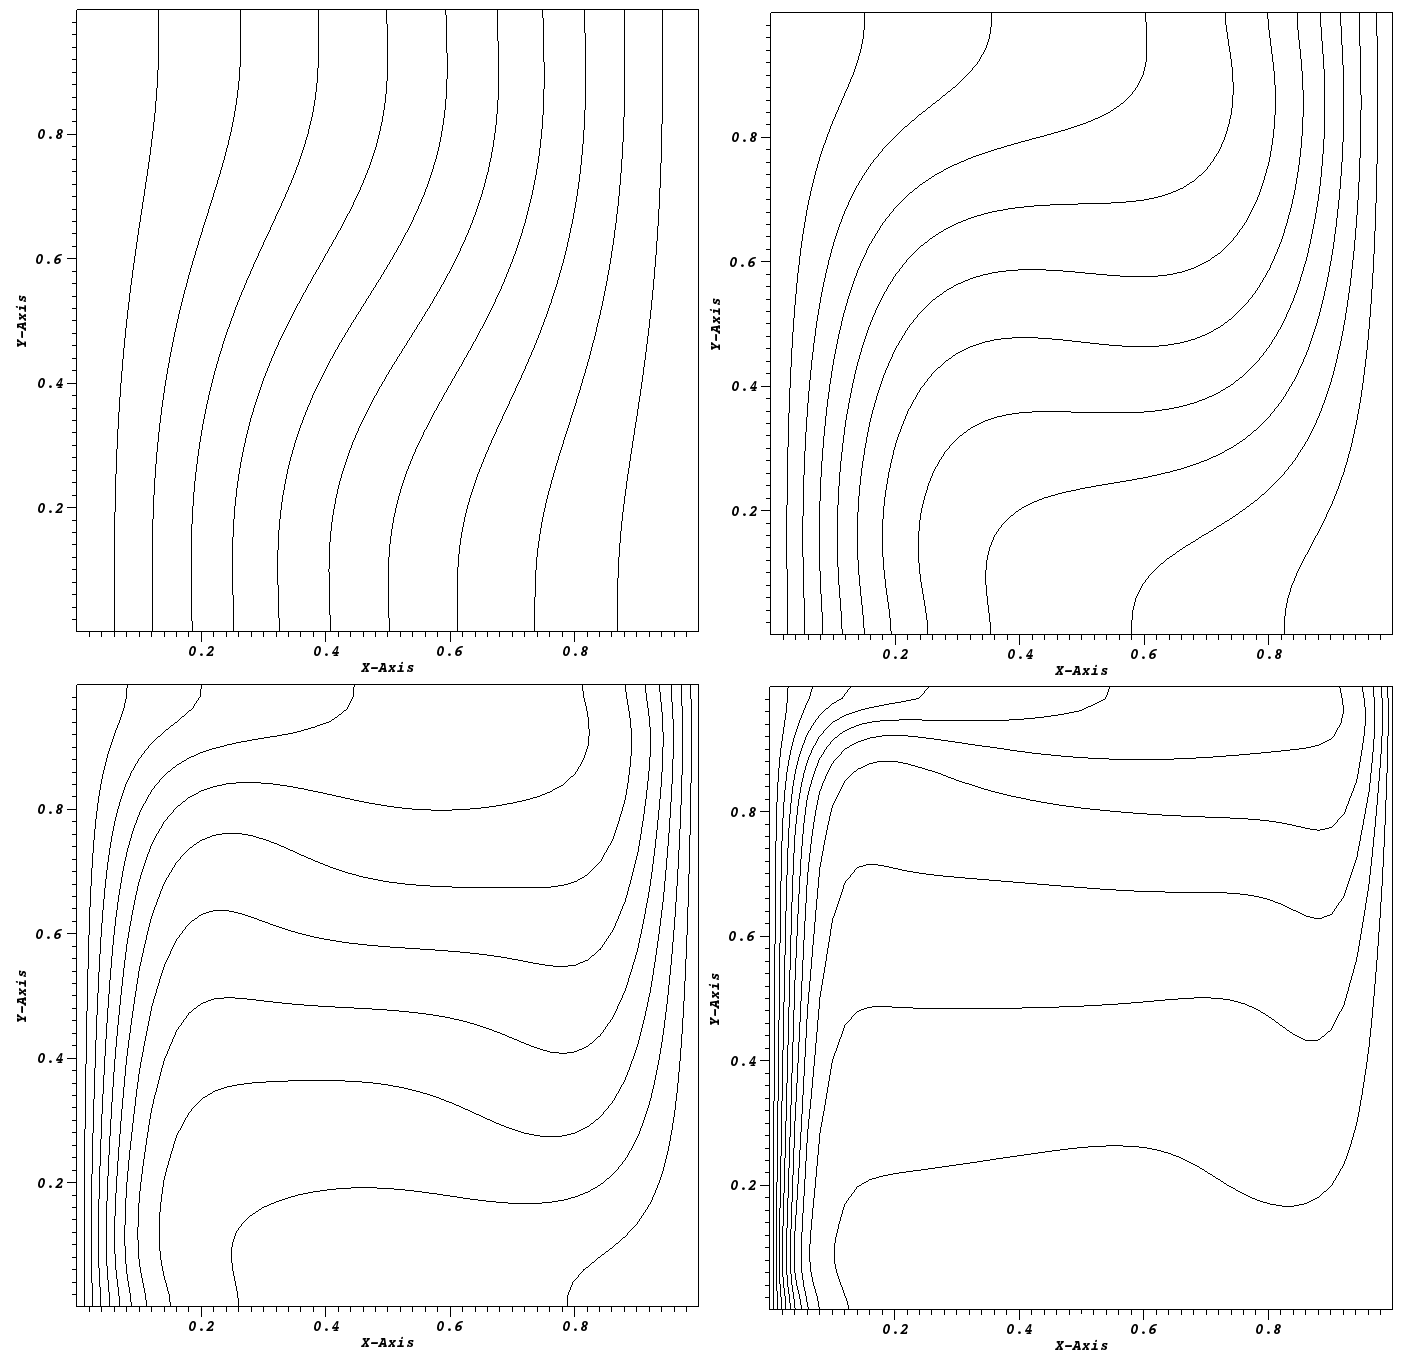
\includegraphics[width=6in]{chapters/nonlinear_problem/convection_isotherms.png}
  \end{center}
  \caption{\textbf{Isotherms from solution to the thermal convection
        cavity problem.} \textit{Top left: Ra = \sn{1}{3}; Top right:
        Ra = \sn{1}{4}; Bottom left: Ra = \sn{1}{5}; Bottom left: Ra =
        \sn{1}{6}. Isotherms on unit temperature scale from 0 to 1
        with divisions of 0.1 for each calculation.}}
  \label{fig:convection_isotherms}
\end{figure}

\clearpage

\subsection{Lid Driven Cavity Problem}
\label{subsec:lid_driven_cavity}
As an extension of the convection problem, the second benchmark
problem given by Ghia \citep{ghia_high-re_1982} adds a driver for the
flow to introduce higher Reynolds numbers into the system, providing
more inertial force to overcome the viscous forces in the fluid. The
setup for this problem is equally simple, containing only the
Dirichlet conditions as given in Figure~\ref{fig:lid_driven_cavity}
and is only applied to the mass and momentum equations on the unit
square.

\begin{figure}[t!]
  \begin{center}
    \scalebox{1.5}{
      \input{chapters/nonlinear_problem/lid_driven_cavity.pdftex_t} }
  \end{center}
  \caption{\textbf{Problem setup for the lid driven cavity benchmark.}
    \textit{Dirichlet conditions of zero are set for the velocity on
      the left and right and bottom while the Dirichlet condition set
      on the top provides a driving force on the fluid.}}
  \label{fig:lid_driven_cavity}
\end{figure}

The top boundary condition will provide a driver for the flow and its
variation will in turn vary the Reynolds number of the fluid. An
increased velocity will generate more inertial forces in the fluid,
which will overcome the viscous forces and again increase the
influence of the nonlinear terms in Eq~(\ref{eq:ns_momentum}). Shadid
used Reynolds numbers up to \sn{1}{4} for this benchmark problem.

Isocurves of the velocity magnitudes are given in
Figure~\ref{fig:driven_velocity_isocurves} for solutions to the lid
driven cavity problem at Reynolds numbers of 100, 300, 500 and
700. Increasing the velocity on the top boundary of the problem drives
up the Reynolds number of the system making it more difficult to
solve. More rotation of the fluid is induced by intertial forces and
we begin to see some additional vortices form besides the primary
vortex in the center of the box.

\begin{figure}[t!]
  \begin{center}
    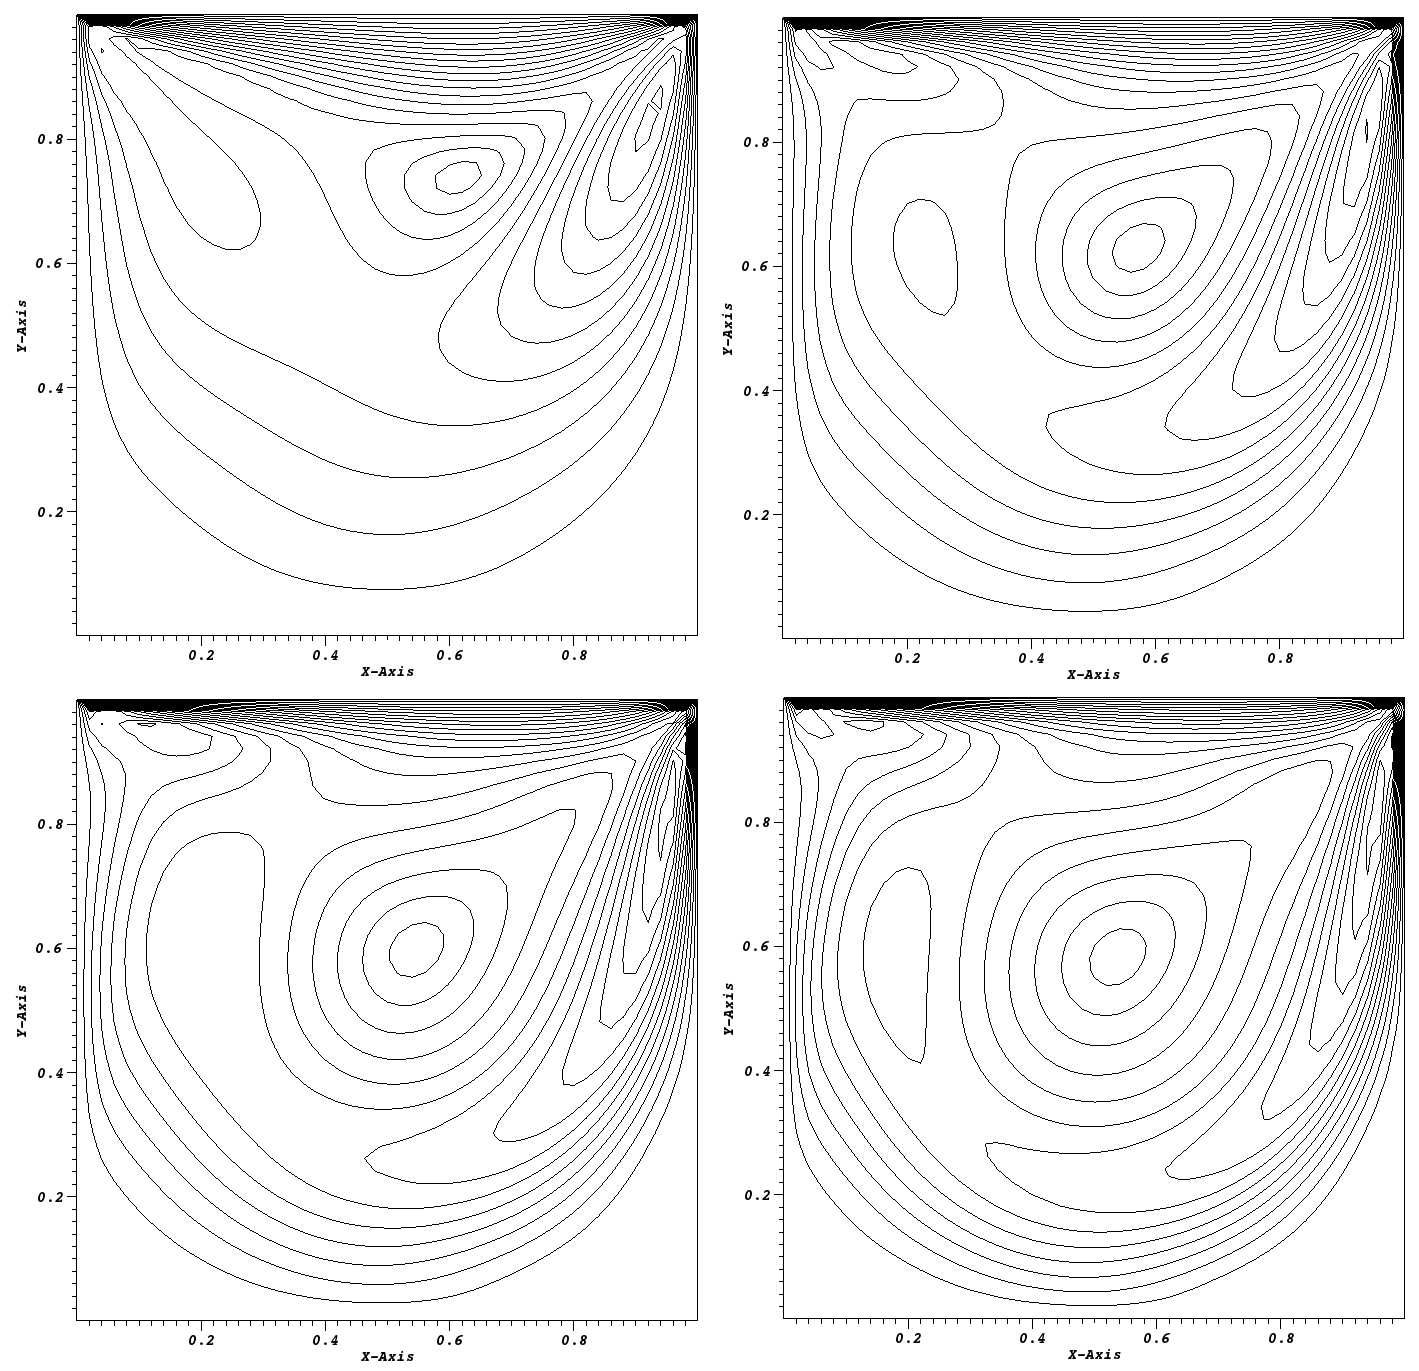
\includegraphics[width=6in]{chapters/nonlinear_problem/driven_velocity_isocurves.png}
  \end{center}
  \caption{\textbf{Velocity magnitude isocurves from solution to the
      thermal convection cavity problem.} \textit{Top left: Re = 100;
      Top right: Re= 300; Bottom left: Re = 500; Bottom left: Re =
      700. Isocurves on unit velocity scale from 0 to 1 with divisions
      of 0.05 for each calculation.}}
  \label{fig:driven_velocity_isocurves}
\end{figure}

\clearpage

%%---------------------------------------------------------------------------%%
\section{FANM Verification\ }
\label{sec:fanm_verification}

For each of the benchmark problems, we will present the results of
computations using FANM and directly compare them to results using a
Newton-Krylov method in order to verify the correctness of FANM and
its applicability to fluid problems. For each case, we will compare
the global minimum, maximum, and average values for fluid velocity,
pressure, and temperature where applicable. In addition, we will
report the tolerance to which the nonlinear residual was converged.

Given the difficulty of these benchmark problems, the linear solve at
each Newton step was preconditioned with an algebraic multigrid
method, a common technique for preconditioning these equations
\citep{ghia_high-re_1982,evans_enhanced_2007}. For FANM, this
preconditioning was required to reduce the spectral radius of the
Jacobian operators generated at each Newton step and for the
Newton-Krylov solutions this preconditioning was required to obtain
good convergence properties although not necessary for
convergence. For every benchmark calculation, both FANM and
Newton-Krylov were preconditioned with the same multigrid parameters
such that the conditioning of the system would not be a factor in the
verification of the method or the perfomance comparison in the
following section.

As with the radiation transport calculations in the previous chapter,
algrebraic preconditioning with the multigrid method results in dense
linear systems. To mitigate this, the reduced domain approximation was
again applied to the Monte Carlo solution within the MCSA solve
occuring at each nonlinear iteration. The values used for the
approximation will be given for each benchmark problem. Without
multigrid preconditioning or too small of a reduced domain fill level,
the residual in MCSA was observed to stagnate. Typically this happens
because the Richardson iteration will damp the higher order error
modes on the scale of the computational grid used to solve the problem
but will miss lower order error modes. In terms of Monte Carlo, this
stagnation manifests itself in histories that simply do no terminate
and therefore no solution is acquired.

Results in this and the following section were produced by the Drekar
multiphysics code base being developed at Sandia National Laboratories
for fluid flow and other multiple physics simulations
\citep{pawlowski_drekar_2012}. Drekar is a massively parallel physics
framework that utilizes Newton-Krylov methods to generate a fully
consistent solution scheme for the Navier-Stokes equations among other
systems with Jacobian generation through automatic differentiation. To
achieve these results, a Monte Carlo solver generated for this work
was injected into the nonlinear toolchain within Drekar to form an
implementation of the FANM method. For the Newton-Krylov solutions,
the same production implementation of GMRES from the Trilinos
scientific computing library Aztec \citep{heroux_overview_2005} used
for the verification of MCSA for the $SP_N$ solutions in the previous
chapter was also used here as a means of comparison.

\subsection{Thermal Convection Cavity Results}
\label{subsec:thermal_convection_verification}

A Drekar model of thermal convection cavity problem was solved using
both the Newton-Krylov solver and a FANM solver for Rayleigh numbers
of \sn{1}{3}, \sn{1}{4}, \sn{1}{5} and
\sn{1}{6}. Table~\ref{tab:thermal_convection_parameters} gives the
physical parameters of the problem and
Table~\ref{tab:convection_mcsa_parameters} gives the MCSA solver
parameters used within the FANM method. Variation in the Rayleigh
number of the system was achieved by keeping the parameters given in
Table~\ref{tab:thermal_convection_parameters} and varying temperature
of the hot side of the cavity. In addition to multigrid
preconditioning for the linear solution at each Newton step,
backtracking as outlined in Shadid's work \citep{shadid_inexact_1997}
was used as a means of globalization assisting the Newton correction
computation while the forcing term was computed using method 2 from
Shadid's work.

\begin{table}[h!]
  \begin{center}
    \begin{tabular}{lcc}\hline\hline
      \multicolumn{1}{l}{Parameter}& 
      \multicolumn{1}{c}{Value}&
      \multicolumn{1}{c}{Units}\\\hline
      $x_{min}$ & 0.0 & $m$ \\
      $x_{max}$ & 1.0 & $m$ \\
      $y_{min}$ & 0.0 & $m$ \\
      $y_{max}$ & 1.0 & $m$ \\
      $N_x$ & 50 & - \\
      $N_y$ & 50 & - \\
      $DOFs$ & 10404 & - \\
      Initial Temperature & 0.0 & $K$ \\
      Density & 1.0 & $kg / m^3$ \\
      Specific Heat & 1.0 & J / $(kg \times K)$ \\
      Dynamic Viscosity & 0.71 & $N \times s / m^2$ \\
      Thermal Conductivity & 1.0 & $W / (m \times K)$ \\
      Thermal Expansion Coefficient & 1000 & $1 / K$ \\
      Thermal Diffusivity & 1.0 & $m^2 / s$ \\
      Kinematic Viscosity & 0.71 & $m^2 / s$ \\
      Gravitational Acceleration & 10 & $m / s^2$ \\
      Cavity Characteristic Length & 1.0 & $m$ \\
      Prandtl Number & 0.71 & - \\
      %%
      \hline\hline
    \end{tabular}
  \end{center}
  \caption{\textbf{Thermal convection cavity FANM verification model
      problem parameters.}  \textit{The Navier-Stokes equations in 2
      dimensions are used for the model problem. The Rayleigh number
      is varied by modifying the hot boundary temperature to induce
      larger temperature gradients and bouyancy-driven flow.}}
  \label{tab:thermal_convection_parameters}
\end{table}

\begin{table}[h!]
  \begin{center}
    \begin{tabular}{lc}\hline\hline
      \multicolumn{1}{l}{Parameter}& 
      \multicolumn{1}{c}{Value}\\\hline
      Histories & 500,000 per iteration \\
      Weight Cutoff & \sn{1}{-2} \\
      Fixed Point Iteration & Richardson \\
      Estimator & Adjoint Collision \\
      Reduced Domain Fill Level & 200 \\
      %%
      \hline\hline
    \end{tabular}
  \end{center}
  \caption{\textbf{Thermal convection cavity FANM verification MCSA
      solver parameters.} \textit{No relaxation parameters or variance
      reduction techniques were used with MCSA other than the reduced
      domain approximation.}}
  \label{tab:convection_mcsa_parameters}
\end{table}

For the verification, at each Rayleigh number variation the global
minimum, maximum, and average values were required for fluid velocity
in the x and y directions, fluid pressure, and fluid
temperature. Tables~\ref{tab:convection_ra1e3_results},
\ref{tab:convection_ra1e4_results},
\ref{tab:convection_ra1e5_results}, and
\ref{tab:convection_ra1e6_results} give the results of these
computations. It should be noted that the negative pressures computed
are due to a relative pressure being reported. For each of the data
points presented, both Newton-Krylov solutions and FANM solutions
computed identical results for all of these global values.

\begin{table}[h!]
  \begin{center}
    \begin{tabular}{lll}\hline\hline
      \multicolumn{1}{l}{Parameter}& 
      \multicolumn{1}{l}{Newton-Krylov Result}&
      \multicolumn{1}{l}{FANM Result}\\
      \hline
      Average $U_x$ & -1.288835730E-05 & -1.288835730E-05 \\
      Minimum $U_x$ & -3.677243960E+00 & -3.677243960E+00 \\
      Maximum $U_x$ & 3.688908550E+00 & 3.688908550E+00 \\
      \hline
      Average $U_y$ & 3.403670530E-02 & 3.403670530E-02 \\
      Minimum $U_y$ & -3.721178580E+00 & -3.721178580E+00 \\
      Maximum $U_y$ & 3.791483420E+00 & 3.791483420E+00 \\
      \hline
      Average $P$ & 2.345554770E+02 & 2.345554770E+02 \\
      Minimum $P$ & -5.509779180E+00 & -5.509779180E+00 \\
      Maximum $P$ & 4.994885560E+02 & 4.994885560E+02 \\
      \hline
      Average $T$ & 3.595148700E-02 & 3.595148700E-02 \\
      Minimum $T$ & 2.092448340E-04 & 2.092448340E-04 \\
      Maximum $T$ & 7.178874510E-02 & 7.178874510E-02 \\
      %%
      \hline\hline
    \end{tabular}
  \end{center}
  \caption{\textbf{Thermal convection cavity FANM verification for a
      Rayleigh number of \sn{1}{3}.} \textit{The values reported are
      global minima, maxima, and averages for each variable in the
      problem. The velocity is given in components in the $x$ and $y$
      directions.}}
  \label{tab:convection_ra1e3_results}
\end{table}

\begin{table}[h!]
  \begin{center}
    \begin{tabular}{lll}\hline\hline
      \multicolumn{1}{l}{Parameter}& 
      \multicolumn{1}{l}{Newton-Krylov Result}&
      \multicolumn{1}{l}{FANM Result}\\
      \hline
      Average $U_x$ & -7.489201240E-04 & -7.489201240E-04 \\
      Minimum $U_x$ & -1.607318000E+01 & -1.607318000E+01 \\
      Maximum $U_x$ & 1.669098270E+01 & 1.669098270E+01 \\
      \hline
      Average $U_y$ & 3.377624420E-01 & 3.377624420E-01 \\
      Minimum $U_y$ & -1.932174800E+01 & -1.932174800E+01 \\
      Maximum $U_y$ & 2.047326820E+01 & 2.047326820E+01 \\
      \hline
      Average $P$ & 1.861894950E+03 & 1.861894950E+03 \\
      Minimum $P$ & -3.353416240E+01 & -3.353416240E+01 \\
      Maximum $P$ & 4.440642810E+03 & 4.440642810E+03 \\
      \hline
      Average $T$ & 3.510568440E-01 & 3.510568440E-01 \\
      Minimum $T$ & 2.092448340E-04 & 2.092448340E-04 \\
      Maximum $T$ & 7.178874510E-02 & 7.178874510E-02 \\
      %%
      \hline\hline
    \end{tabular}
  \end{center}
  \caption{\textbf{Thermal convection cavity FANM verification for a
      Rayleigh number of \sn{1}{4}.} \textit{The values reported are
      global minima, maxima, and averages for each variable in the
      problem. The velocity is given in components in the $x$ and $y$
      directions.}}
  \label{tab:convection_ra1e4_results}
\end{table}

\begin{table}[h!]
  \begin{center}
    \begin{tabular}{lll}\hline\hline
      \multicolumn{1}{l}{Parameter}& 
      \multicolumn{1}{l}{Newton-Krylov Result}&
      \multicolumn{1}{l}{FANM Result}\\
      \hline
      Average $U_x$ & -2.043639370E-02 & -2.043639370E-02 \\
      Minimum $U_x$ & -3.814922470E+01 & -3.814922470E+01 \\
      Maximum $U_x$ & -3.814922470E+01 & -3.814922470E+01 \\
      \hline
      Average $U_y$ & 2.774864300E+00 & 2.774864300E+00 \\
      Minimum $U_y$ & -6.038682990E+01 & -6.038682990E+01 \\
      Maximum $U_y$ & 7.873873560E+01 & 7.873873560E+01 \\
      \hline
      Average $P$ & 1.324208380E+04 & 1.324208380E+04 \\
      Minimum $P$ & -1.390235490E+02 & -1.390235490E+02 \\
      Maximum $P$ & 3.559215530E+04 & 3.559215530E+04 \\
      \hline
      Average $T$ & 3.027827770E+00 & 3.027827770E+00 \\
      Minimum $T$ & 1.626405740E-02 & 1.626405740E-02 \\
      Maximum $T$ & 7.162571130E+00 & 7.162571130E+00 \\
      %%
      \hline\hline
    \end{tabular}
  \end{center}
  \caption{\textbf{Thermal convection cavity FANM verification for a
      Rayleigh number of \sn{1}{5}.} \textit{The values reported are
      global minima, maxima, and averages for each variable in the
      problem. The velocity is given in components in the $x$ and $y$
      directions.}}
  \label{tab:convection_ra1e5_results}
\end{table}

\begin{table}[h!]
  \begin{center}
    \begin{tabular}{lll}\hline\hline
      \multicolumn{1}{l}{Parameter}& 
      \multicolumn{1}{l}{Newton-Krylov Result}&
      \multicolumn{1}{l}{FANM Result}\\
      \hline
      Average $U_x$ & -1.802569840E-01 & -1.802569840E-01 \\
      Minimum $U_x$ & -6.292084130E+01 & -6.292084130E+01 \\
      Maximum $U_x$ & 2.951113240E+02 & 2.951113240E+02 \\
      \hline
      Average $U_y$ & 1.336398550E+01 & 1.336398550E+01 \\
      Minimum $U_y$ & -1.345663290E+02 & -1.345663290E+02 \\
      Maximum $U_y$ & 3.227873890E+02 & 3.227873890E+02 \\
      \hline
      Average $P$ & 6.354313840E+04 & 6.354313840E+04 \\
      Minimum $P$ & -1.356309630E+02 & -1.356309630E+02 \\
      Maximum $P$ & 2.316308730E+05 & 2.316308730E+05 \\
      \hline
      Average $T$ & 1.780727610E+01 & 1.780727610E+01 \\
      Minimum $T$ & 8.265788890E-02 & 8.265788890E-02 \\
      Maximum $T$ & 7.098873170E+01 & 7.098873170E+01 \\
      %%
      \hline\hline
    \end{tabular}
  \end{center}
  \caption{\textbf{Thermal convection cavity FANM verification for a
      Rayleigh number of \sn{1}{6}.} \textit{The values reported are
      global minima, maxima, and averages for each variable in the
      problem. The velocity is given in components in the $x$ and $y$
      directions.}}
  \label{tab:convection_ra1e6_results}
\end{table}

\begin{table}[h!]
  \begin{center}
    \begin{tabular}{lcc}\hline\hline
      \multicolumn{1}{l}{Rayleigh Number}& 
      \multicolumn{1}{c}{Newton Krylov $||\ve{F(\ve{u})}||$}&
      \multicolumn{1}{c}{FANM $||\ve{F(\ve{u})}||$}\\
      \hline
      \sn{1}{3} & \sn{4.542}{-14} & \sn{1.208}{-14} \\
      \sn{1}{4} & \sn{1.045}{-12} & \sn{7.012}{-13} \\
      \sn{1}{5} & \sn{1.784}{-12} & \sn{1.059}{-12} \\
      \sn{1}{6} & \sn{3.404}{-12} & \sn{3.479}{-12} \\
      %%
      \hline\hline
    \end{tabular}
  \end{center}
  \caption{\textbf{Thermal convection cavity nonlinear residual norm
      achieved convergence.} \textit{The results presented here were
      obtained from the benchmark verification calculations.}}
  \label{tab:convection_residual_norm_comparison}
\end{table}

\clearpage

\subsection{Lid Driven Cavity Results}
\label{subsec:lid_driven_verification}

A Drekar model of thermal convection cavity problem was solved using
both the Newton-Krylov solver and a FANM solver for Reynolds numbers
of 100, 300, 500, and
700. Table~\ref{tab:thermal_convection_parameters} gives the physical
parameters of the problem and
Table~\ref{tab:convection_mcsa_parameters} gives the MCSA solver
parameters used within the FANM method. Variation in the Reynolds
number of the system was achieved by keeping the parameters given in
Table~\ref{tab:thermal_convection_parameters} and varying the fluid
velocity in the $x$ direction on the top boundary. In addition to
multigrid preconditioning for the linear solution at each Newton step,
a polynomial line search method was used as a means of globalization
assisting the Newton correction computation as outlined by Pawlowski
in \citep{pawlowski_globalization_2006} while the forcing term was
computed using method 2 from Shadid's work
\citep{shadid_inexact_1997}.

\begin{table}[h!]
  \begin{center}
    \begin{tabular}{lcc}\hline\hline
      \multicolumn{1}{l}{Parameter}& 
      \multicolumn{1}{c}{Value}&
      \multicolumn{1}{c}{Units}\\\hline
      $x_{min}$ & 0.0 & $m$ \\
      $x_{max}$ & 1.0 & $m$ \\
      $y_{min}$ & 0.0 & $m$ \\
      $y_{max}$ & 1.0 & $m$ \\
      $N_x$ & 50 & - \\
      $N_y$ & 50 & - \\
      $DOFs$ & 7803 & - \\
      Density & 1.0 & $kg / m^3$ \\
      Dynamic Viscosity & 0.71 & $N \times s / m^2$ \\
      Kinematic Viscosity & 0.71 & $m^2 / s$ \\
      Gravitational Acceleration & 10 & $m / s^2$ \\
      Cavity Characteristic Length & 1.0 & $m$ \\
      %%
      \hline\hline
    \end{tabular}
  \end{center}
  \caption{\textbf{Lid driven cavity FANM verification model
      problem parameters.}  \textit{The Navier-Stokes equations in 2
      dimensions are used for the model problem. The Reynolds number
      is varied by modifying the velocity magnitude on the upper
      boundary to induce flow driven by inertial forces.}}
  \label{tab:lid_driven_parameters}
\end{table}

\begin{table}[h!]
  \begin{center}
    \begin{tabular}{lc}\hline\hline
      \multicolumn{1}{l}{Parameter}& 
      \multicolumn{1}{c}{Value}\\\hline
      Weight Cutoff & \sn{1}{-2} \\
      Fixed Point Iteration & Richardson \\
      Estimator & Adjoint Collision \\
      Histories, Re=100 & 500,000 per iteration \\
      Histories, Re=300 & 500,000 per iteration \\
      Histories, Re=500 & 500,000 per iteration \\
      Histories, Re=700 & 1,000,000 per iteration \\
      Reduced Domain Fill Level, Re=100 & 200 \\
      Reduced Domain Fill Level, Re=300 & 200 \\
      Reduced Domain Fill Level, Re=500 & 200 \\
      Reduced Domain Fill Level, Re=700 & 300 \\
      %%
      \hline\hline
    \end{tabular}
  \end{center}
  \caption{\textbf{Lid driven cavity FANM verification MCSA solver
      parameters.} \textit{No relaxation parameters or variance
      reduction techniques were used with MCSA other than the reduced
      domain approximation. Different values of fill level for the
      reduced domain approximation and histories per iteration were
      used at different Reynolds numbers due to convergence
      requirements.}}
  \label{tab:driven_mcsa_parameters}
\end{table}

In the literature on this benchmark, solutions at Reynolds numbers of
up to \sn{1}{4} were achieved using a variety of nonlinear solution
techniques. With the FANM method, at Reynolds numbers above 700,
convergence of the linear iterations could not be achieved regardless
of how agressive the multigrid preconditioner was set. In these cases,
the Jacobian operators are ill-conditioned enough that even GMRES
converges slowly relative to the thermal convection cavity
benchmark. Therefore, the spectral radius limitation on MCSA is
extremely prohibitive in this case and others were transport driven by
intertial forces is dominant. Because of this, only solutions to the
lid driven cavity benchmark at Reynolds numbers of up to 700 are
presented.

For the verification, at each Reynolds number variation the global
minimum, maximum, and average values were required for fluid velocity
in the x and y directions, fluid pressure, and fluid
temperature. Tables~\ref{tab:driven_re100_results},
\ref{tab:driven_re300_results}, \ref{tab:driven_re500_results}, and
\ref{tab:driven_re700_results} give the results of these
computations. It should be noted that the negative pressures computed
are due to a relative pressure being reported. For each of the data
points presented, both Newton-Krylov solutions and FANM solutions
computed identical results for all of these global values.

\begin{table}[h!]
  \begin{center}
    \begin{tabular}{lll}\hline\hline
      \multicolumn{1}{l}{Parameter}& 
      \multicolumn{1}{l}{Newton-Krylov Result}&
      \multicolumn{1}{l}{FANM Result}\\
      \hline
      Average $U_x$ & 1.165632320E-01 & 1.165632320E-01 \\
      Minimum $U_x$ & -2.423642920E+01 & -2.423642920E+01 \\
      Maximum $U_x$ & 9.742670880E+01 & 9.742670880E+01 \\
      \hline
      Average $U_y$ & 2.038480420E-02 & 2.038480420E-02 \\
      Minimum $U_y$ & -5.266315430E+01 & -5.266315430E+01 \\
      Maximum $U_y$ & 2.720044160E+01 & 2.720044160E+01 \\
      \hline
      Average $P$ & -1.656193900E+02 & -1.656193900E+02 \\
      Minimum $P$ & -9.635479370E+03 & -9.635479370E+03 \\
      Maximum $P$ & 1.854517020E+04 & 1.854517020E+04 \\
      %%
      \hline\hline
    \end{tabular}
  \end{center}
  \caption{\textbf{Lid driven cavity FANM verification for a Reynolds
      number of 100.} \textit{The values reported are global minima,
      maxima, and averages for each variable in the problem. The
      velocity is given in components in the $x$ and $y$ directions.}}
  \label{tab:driven_re100_results}
\end{table}

\begin{table}[h!]
  \begin{center}
    \begin{tabular}{lll}\hline\hline
      \multicolumn{1}{l}{Parameter}& 
      \multicolumn{1}{l}{Newton-Krylov Result}&
      \multicolumn{1}{l}{FANM Result}\\
      \hline
      Average $U_x$ & 3.382078040E-01 & 3.382078040E-01 \\
      Minimum $U_x$ & -9.467140360E+01 & -9.467140360E+01 \\
      Maximum $U_x$ & 2.895885380E+02 & 2.895885380E+02 \\
      \hline
      Average $U_y$ & 8.780242440E-02 & 8.780242440E-02 \\
      Minimum $U_y$ & -1.830156060E+02 & -1.830156060E+02 \\
      Maximum $U_y$ & 8.827373340E+01 & 8.827373340E+01 \\
      \hline
      Average $P$ & -2.830380160E+03 & -2.830380160E+03 \\
      Minimum $P$ & -2.352177540E+04 & -2.352177540E+04 \\
      Maximum $P$ & 9.254997120E+04 & 9.254997120E+04 \\
      %%
      \hline\hline
    \end{tabular}
  \end{center}
  \caption{\textbf{Lid driven cavity FANM verification for a Reynolds
      number of 300.} \textit{The values reported are global minima,
      maxima, and averages for each variable in the problem. The
      velocity is given in components in the $x$ and $y$ directions.}}
  \label{tab:driven_re300_results}
\end{table}

\begin{table}[h!]
  \begin{center}
    \begin{tabular}{lll}\hline\hline
      \multicolumn{1}{l}{Parameter}& 
      \multicolumn{1}{l}{Newton-Krylov Result}&
      \multicolumn{1}{l}{FANM Result}\\
      \hline
      Average $U_x$ & 5.098921320E-01 & 5.098921320E-01 \\
      Minimum $U_x$ & -1.731861690E+02 & -1.731861690E+02 \\
      Maximum $U_x$ & 4.789146040E+02 & 4.789146040E+02 \\
      \hline
      Average $U_y$ & 1.365493140E-01 & 1.365493140E-01 \\
      Minimum $U_y$ & -3.170930360E+02 & -3.170930360E+02 \\
      Maximum $U_y$ & 1.655401440E+02 & 1.655401440E+02 \\
      \hline
      Average $P$ & -9.378317550E+03 & -9.378317550E+03 \\
      Minimum $P$ & -4.155215280E+04 & -4.155215280E+04 \\
      Maximum $P$ & 2.058742010E+05 & 2.058742010E+05 \\
      %%
      \hline\hline
    \end{tabular}
  \end{center}
  \caption{\textbf{Lid driven cavity FANM verification for a
      Reynolds number of 500.} \textit{The values reported are
      global minima, maxima, and averages for each variable in the
      problem. The velocity is given in components in the $x$ and $y$
      directions.}}
  \label{tab:driven_re500_results}
\end{table}

\begin{table}[h!]
  \begin{center}
    \begin{tabular}{lll}\hline\hline
      \multicolumn{1}{l}{Parameter}& 
      \multicolumn{1}{l}{Newton-Krylov Result}&
      \multicolumn{1}{l}{FANM Result}\\
      \hline
      Average $U_x$ & 6.479541170E-01 & 6.479541170E-01 \\
      Minimum $U_x$ & -2.550685400E+02 & -2.550685400E+02 \\
      Maximum $U_x$ & 6.663054900E+02 & 6.663054900E+02 \\
      \hline
      Average $U_y$ & 1.833690840E-01 & 1.833690840E-01 \\
      Minimum $U_y$ & -4.491052980E+02 & -4.491052980E+02 \\
      Maximum $U_y$ & 2.474376340E+02 & 2.474376340E+02 \\
      \hline
      Average $P$ & 1.833690840E-01 & 1.833690840E-01 \\
      Minimum $P$ & -6.241704500E+04 & -6.241704500E+04 \\
      Maximum $P$ & 3.518174810E+05 & 3.518174810E+05 \\
      %%
      \hline\hline
    \end{tabular}
  \end{center}
  \caption{\textbf{Lid driven cavity FANM verification for a Reynolds
      number of 700.} \textit{The values reported are global minima,
      maxima, and averages for each variable in the problem. The
      velocity is given in components in the $x$ and $y$ directions.}}
  \label{tab:driven_re700_results}
\end{table}

\begin{table}[h!]
  \begin{center}
    \begin{tabular}{lcc}\hline\hline
      \multicolumn{1}{l}{Reynolds Number}& 
      \multicolumn{1}{c}{Newton Krylov $||\ve{F(\ve{u})}||$}&
      \multicolumn{1}{c}{FANM $||\ve{F(\ve{u})}||$}\\
      \hline
      100 & \sn{5.453}{-14} & \sn{6.577}{-14} \\
      300 & \sn{2.537}{-13} & \sn{2.779}{-13} \\
      500 & \sn{6.367}{-13} & \sn{6.252}{-13} \\
      700 & \sn{9.159}{-13} & \sn{1.282}{-12} \\
      %%
      \hline\hline
    \end{tabular}
  \end{center}
  \caption{\textbf{Lid driven cavity nonlinear residual norm
      achieved convergence.} \textit{The results presented here were
      obtained from the benchmark verification calculations.}}
  \label{tab:driven_residual_norm_comparison}
\end{table}

\clearpage

%%---------------------------------------------------------------------------%%
\section{FANM Performance Comparison to Conventional Methods\ }
\label{sec:fanm_comparison}

Using the benchmarks from the verification, we now compare the
performance of the FANM method against a conventional Krylov
method. For each benchmark, we will analyze the iterative performance
of both the Newton solver and the linear solver used to compute the
correction vector at each step. In addition, timing results will be discussed

\subsection{Thermal Convection Cavity Results}
\label{subsec:thermal_convection_comparison}


\begin{table}[h!]
  \begin{center}
    \begin{tabular}{lcc}\hline\hline
      \multicolumn{1}{l}{Rayleigh Number}& 
      \multicolumn{1}{c}{Newton-Krylov Iterations}&
      \multicolumn{1}{c}{FANM Iterations}\\
      \hline
      \sn{1}{3} & 5 & 5 \\
      \sn{1}{4} & 7 & 7 \\
      \sn{1}{5} & 9 & 10 \\
      \sn{1}{6} & 11 & 11 \\
      %%
      \hline\hline
    \end{tabular}
  \end{center}
  \caption{\textbf{Thermal convection cavity nonlinear iteration
      results for the performance comparison.} \textit{The results
      presented here were obtained from the benchmark verification
      calculations.}}
  \label{tab:convection_nonlinear_iter_comparison}
\end{table}

\begin{table}[h!]
  \begin{center}
    \begin{tabular}{lcc}\hline\hline
      \multicolumn{1}{l}{Rayleigh Number}& 
      \multicolumn{1}{c}{GMRES Iterations}&
      \multicolumn{1}{c}{MCSA Iterations}\\
      \hline
      \sn{1}{3} & 23 & 18 \\
      \sn{1}{4} & 23 & 17 \\
      \sn{1}{5} & 25 & 20 \\
      \sn{1}{6} & 39 & 25 \\
      %%
      \hline\hline
    \end{tabular}
  \end{center}
  \caption{\textbf{Thermal convection cavity total sum of linear
      iterations for all nonlinear iterations.} \textit{The results
      presented here were obtained from the benchmark verification
      calculations.}}
  \label{tab:convection_linear_iter_comparison}
\end{table}

\begin{table}[h!]
  \begin{center}
    \begin{tabular}{lcc}\hline\hline
      \multicolumn{1}{l}{Rayleigh Number}& 
      \multicolumn{1}{c}{Newton-Krylov Speedup}\\
      \hline
      \sn{1}{3} & 338 \\
      \sn{1}{4} & 336 \\
      \sn{1}{5} & 346 \\
      \sn{1}{6} & 465 \\
      %%
      \hline\hline
    \end{tabular}
  \end{center}
  \caption{\textbf{Thermal convection cavity Newton-Krylov speedup
      over FANM method.} \textit{Speedup values are rounded to the
      nearest integer. The results presented here were obtained from
      the benchmark verification calculations.}}
  \label{tab:convection_speedup_comparison}
\end{table}

\clearpage

\subsection{Lid Driven Cavity Results}
\label{subsec:lid_driven_comparison}

\begin{table}[h!]
  \begin{center}
    \begin{tabular}{lcc}\hline\hline
      \multicolumn{1}{l}{Reynolds Number}& 
      \multicolumn{1}{c}{Newton-Krylov Iterations}&
      \multicolumn{1}{c}{FANM Iterations}\\
      \hline
      100 & 6 & 6 \\
      300 & 9 & 9 \\
      500 & 11 & 11 \\
      700 & 14 & 10 \\
      %%
      \hline\hline
    \end{tabular}
  \end{center}
  \caption{\textbf{Lid driven cavity nonlinear iteration
      results for the performance comparison.} \textit{The results
      presented here were obtained from the benchmark verification
      calculations.}}
  \label{tab:driven_nonlinear_iter_comparison}
\end{table}

\begin{table}[h!]
  \begin{center}
    \begin{tabular}{lcc}\hline\hline
      \multicolumn{1}{l}{Reynolds Number}& 
      \multicolumn{1}{c}{GMRES Iterations}&
      \multicolumn{1}{c}{MCSA Iterations}\\
      \hline
      100 & 27 & 42 \\
      300 & 35 & 52 \\
      500 & 41 & 56 \\
      700 & 21 & 14 \\
      %%
      \hline\hline
    \end{tabular}
  \end{center}
  \caption{\textbf{Lid driven cavity total sum of linear
      iterations for all nonlinear iterations.} \textit{The results
      presented here were obtained from the benchmark verification
      calculations.}}
  \label{tab:driven_linear_iter_comparison}
\end{table}

\begin{table}[h!]
  \begin{center}
    \begin{tabular}{lcc}\hline\hline
      \multicolumn{1}{l}{Reynolds Number}& 
      \multicolumn{1}{c}{Newton-Krylov Speedup}\\
      \hline
      100 & 299 \\
      300 & 322 \\
      500 & 288 \\
      700 & 488 \\
      %%
      \hline\hline
    \end{tabular}
  \end{center}
  \caption{\textbf{Lid driven cavity Newton-Krylov speedup
      over FANM method.} \textit{Speedup values are rounded to the
      nearest integer. The results presented here were obtained from
      the benchmark verification calculations.}}
  \label{tab:driven_speedup_comparison}
\end{table}
